\chapter{Architecture et conception}
\label{chap:architecture}

\section{Introduction}
Ce chapitre décrit l'architecture du jumeau numérique couche par couche, en justifiant chaque choix technologique. Il détaille ensuite le modèle de données : le registre des signaux, la structure des messages \gls{mqtt}, l'historien et le cycle de vie d'une donnée.

\section{Vue d'ensemble}
Le système est organisé en cinq couches (figure~\ref{fig:archi}). Deux sources de télémétrie alimentent un même broker MQTT : la \textbf{relecture des historiques du procédé} et une \textbf{chaîne industrielle} KEPServerEX -- Node-RED qui reproduit le trajet réel d'une mesure, de l'automate jusqu'au réseau. Toutes les autres briques consomment ces messages sans savoir d'où ils viennent : on peut ainsi remplacer le simulateur par une vraie usine sans modifier le reste du système.

\begin{figure}[H]
\centering
\resizebox{\textwidth}{!}{\begin{tikzpicture}[
  n/.style={draw,rounded corners=2pt,fill=white,font=\scriptsize,align=center,minimum width=2.8cm,minimum height=0.9cm},
  db/.style={cylinder,shape border rotate=90,aspect=0.2,draw,fill=white,font=\scriptsize,align=center,minimum width=2.5cm,minimum height=1.2cm},
  zone/.style={draw,dashed,rounded corners=6pt,inner sep=7pt},
  titre/.style={font=\footnotesize\bfseries,anchor=south west,inner sep=2pt},
  f/.style={-{Stealth[length=2mm]},thick,gris},
  lab/.style={font=\tiny,gris,fill=white,inner sep=1pt}]
  % ---- 1. Sources
  \node[n,draw=orange] (kep) at (0,1.2) {KEPServerEX\\45 tags simulés};
  \node[n,draw=orange] (nr)  at (3.6,1.2) {Node-RED\\passerelle IIoT};
  \node[n,draw=orange] (csv) at (0,-0.4) {Historiques CSV\\procédé + santé};
  \node[n,draw=orange] (pub) at (3.6,-0.4) {Publieur Python\\relecture pilotable};
  \draw[f] (kep)--node[lab,above=1pt]{OPC UA}(nr);
  \draw[f] (csv)--(pub);
  \node[zone,draw=orange,fit=(kep)(nr)(csv)(pub)] (z1) {};
  \node[titre,text=orange] at (z1.north west) {1. Sources de télémétrie};
  % ---- 2. Transport + traitement
  \node[n,draw=bleu] (mq)  at (7.9,0.4) {Broker Mosquitto\\MQTT :1883};
  \node[n,draw=bleu,minimum width=3.6cm] (api) at (12.8,0.4) {Backend FastAPI\\telemetry $\cdot$ simulation $\cdot$ assets\\knowledge\_graph $\cdot$ faults $\cdot$ prognosis $\cdot$ auth};
  \draw[f] (nr.east) -- ++(0.5,0) |- ([yshift=2mm]mq.west);
  \draw[f] (pub.east) -- ++(0.5,0) |- ([yshift=-2mm]mq.west);
  \draw[f] (mq)--node[lab,above=2pt]{abonnement}(api);
  \node[zone,draw=bleu,fit=(mq)(api)] (z2) {};
  \node[titre,text=bleu] at (z2.north west) {2. Transport et traitement};
  % ---- 3. Stockage
  \node[db,draw=vert] (hist) at (9.6,-2.6) {Historien\\SQLite};
  \node[db,draw=vert] (neo)  at (12.8,-2.6) {Neo4j\\(ou graphe mémoire)};
  \node[db,draw=vert] (files) at (16.0,-2.6) {CSV de référence\\+ GMAO};
  \draw[f] (api.south) -- (hist.north);
  \draw[f] (api.south) -- (neo.north);
  \draw[f] (api.south) -- (files.north);
  \node[zone,draw=vert,fit=(hist)(neo)(files)] (z3) {};
  \node[titre,text=vert] at (z3.north west) {3. Stockage};
  % ---- 4. IA
  \node[n,draw=rouge] (wi)  at (0.9,-2.6) {Détection des défauts\\10 règles SI\,…\,ALORS};
  \node[n,draw=rouge] (rag) at (4.2,-2.6) {Copilote Graph RAG\\LLM + graphe};
  \node[n,draw=rouge] (xgb) at (2.55,-4.0) {Pronostic\\durée de vie résiduelle};
  \node[zone,draw=rouge,fit=(wi)(rag)(xgb)] (z4) {};
  \node[titre,text=rouge] at (z4.north west) {4. Analyse et aide à la décision};
  \draw[f,<->] (z4.east) -- node[lab,above=2pt]{mesures, graphe, contexte} (z3.west);
  % ---- 5. IHM
  \node[n,draw=violet,minimum width=3.6cm] (react) at (12.8,-5.2) {Application React (SPA)};
  \node[n,draw=violet,minimum width=2.4cm] (syn) at (10.1,-6.5) {Synoptique, défauts\\+ graphe};
  \node[n,draw=violet,minimum width=2.4cm] (d3)  at (12.8,-6.5) {Vue 3D};
  \node[n,draw=violet,minimum width=2.4cm] (mt)  at (15.5,-6.5) {Maintenance, pronostic\\+ copilote};
  \node[zone,draw=violet,fit=(react)(syn)(d3)(mt)] (z5) {};
  \node[titre,text=violet] at (z5.north west) {5. Interface utilisateur};
  \draw[f,<->] (api.east) -- ++(3.0,0) |- node[lab,pos=0.25,right=1pt]{API REST + JWT} (react.east);
\end{tikzpicture}
}
\caption{Architecture globale du jumeau numérique}
\label{fig:archi}
\end{figure}

Le tableau~\ref{tab:5d} rattache chaque élément de l'architecture aux cinq dimensions du modèle de Tao \textit{et al.}~\cite{tao2018}.

\begin{table}[H]
\centering
\caption{Correspondance entre l'architecture et le modèle à cinq dimensions~\cite{tao2018}}
\label{tab:5d}
\begin{tabularx}{\textwidth}{lX}
\toprule
\textbf{Dimension} & \textbf{Éléments du prototype} \\
\midrule
Entité physique & Circuit de broyage représenté par KEPServerEX (automate simulé) et par les historiques du procédé \\
Entité virtuelle & Bilans de matière, graphe de connaissances, règles de diagnostic, modèle de dégradation, modèle 3D \\
Données & Historien SQLite, jeux de données CSV, registre des tags, Neo4j \\
Connexions & OPC UA, MQTT, API REST \\
Services & Synoptique, diagnostic des défauts, fiches équipements, maintenance et pronostic, copilote IA \\
\bottomrule
\end{tabularx}
\end{table}

\section{Couche 1 : sources de télémétrie}

\subsection{Chaîne industrielle KEPServerEX -- Node-RED}
Cette chaîne reproduit le trajet d'une mesure dans une usine réelle :
\begin{itemize}
  \item \textbf{KEPServerEX}~\cite{kepware} joue le rôle de l'automate et de son serveur \gls{opcua}. Le canal \texttt{Circuit\_Broyage}, équipement \texttt{Broyeur\_Boulets}, contient les 45 tags du circuit. Chaque tag est généré par le pilote de simulation (fonction \texttt{RAMP}) et exposé sur le point d'accès \texttt{opc.tcp://localhost:49320}.
  \item \textbf{Node-RED}~\cite{nodered} sert de passerelle \gls{iiot}. Au déploiement, un nœud construit la liste des 45 identifiants OPC UA à partir du registre. Un client OPC UA s'y abonne, puis une fonction associe chaque tag à son topic MQTT et met le message au format attendu par le backend avant de le publier (figure~\ref{fig:nodered}).
\end{itemize}

\begin{figure}[H]
\centering
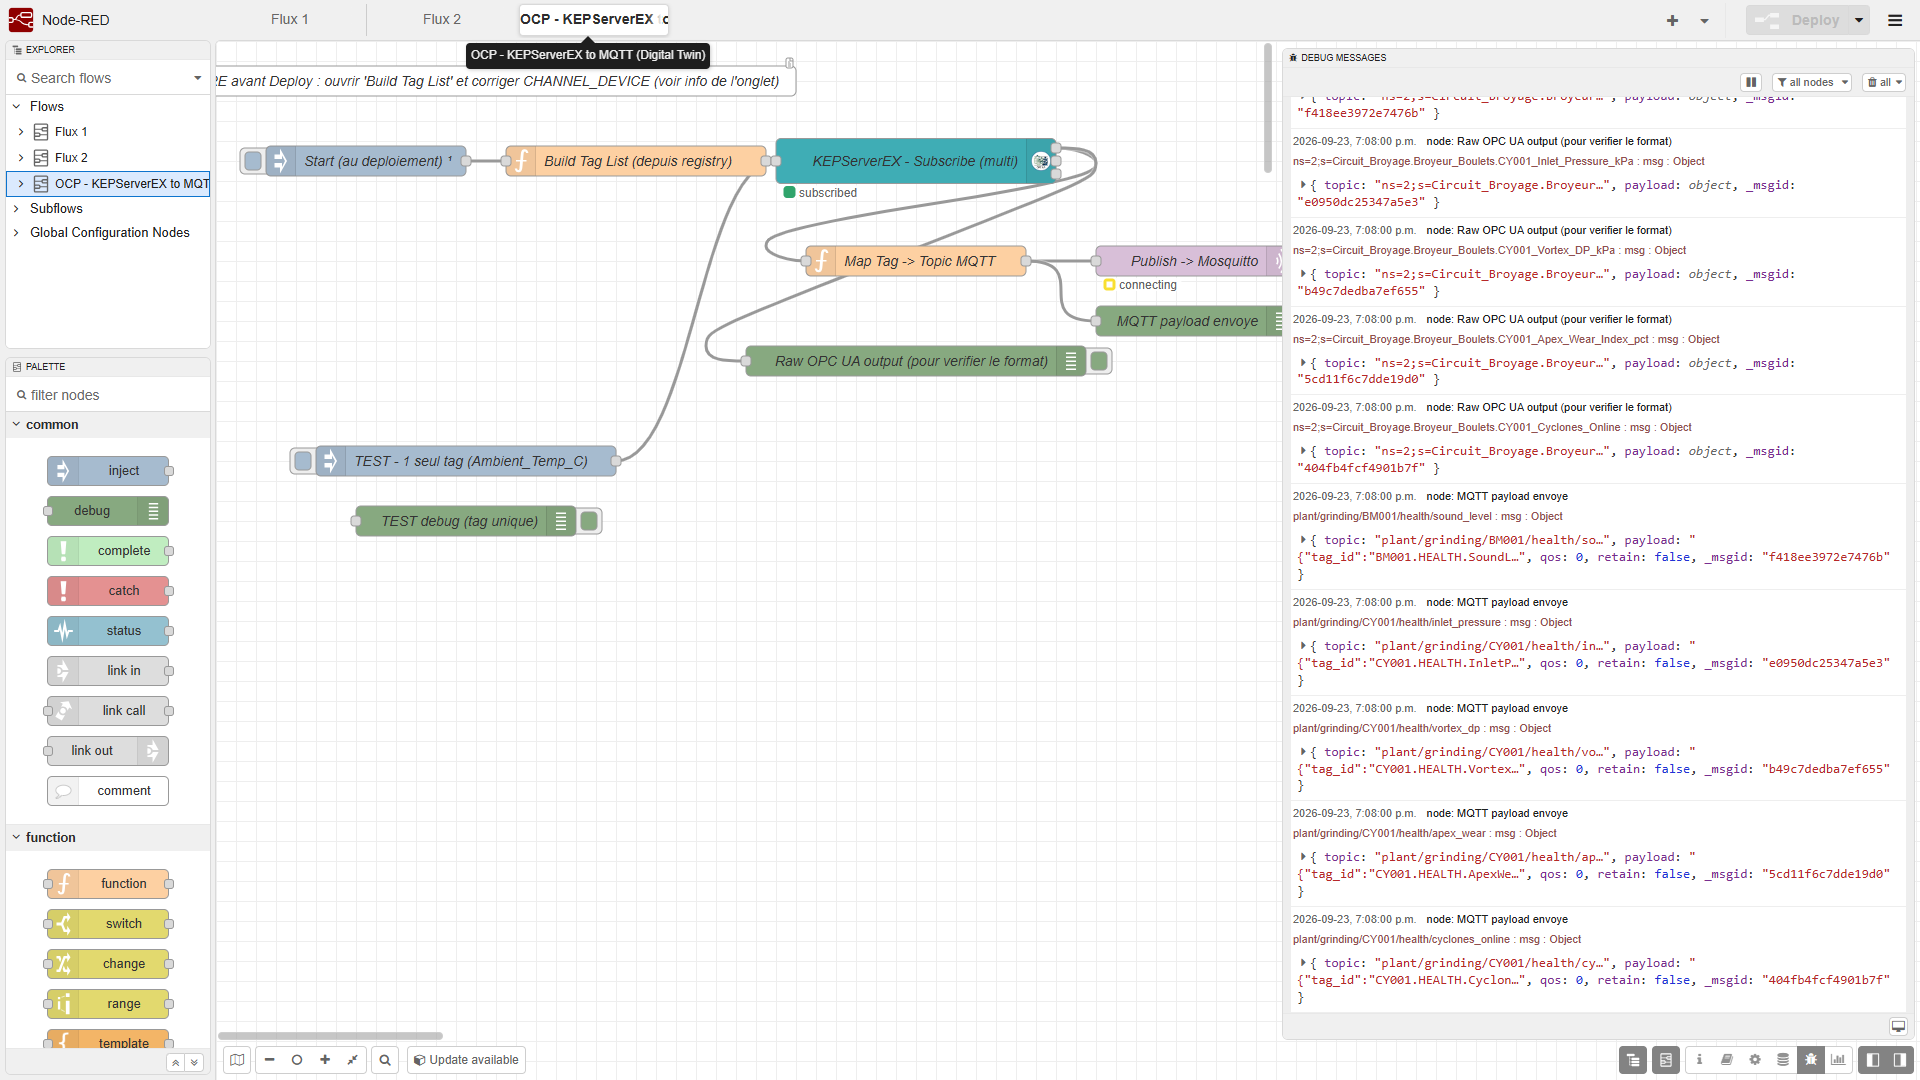
\includegraphics[width=\textwidth]{app_nodered}
\caption{Flux Node-RED «~OCP -- KEPServerEX to MQTT~» : abonnement OPC UA à KEPServerEX (état \textit{subscribed}), mise au format et publication MQTT ; à droite, les messages produits}
\label{fig:nodered}
\end{figure}

\subsection{Relecture des historiques}
La seconde source est un publieur Python, lancé dans son propre conteneur, qui rejoue les historiques du procédé :
\begin{itemize}
  \item 2\,880 mesures de procédé, une toutes les 15 minutes ;
  \item 43\,200 mesures de santé, une par minute.
\end{itemize}
Les deux fichiers couvrent le mois de juillet 2026. Le publieur s'appuie sur le registre des tags pour publier chaque colonne sur son topic. Il écoute aussi le topic de contrôle \texttt{plant/simulation/control}, ce qui permet de démarrer, suspendre ou accélérer la relecture depuis l'interface (jusqu'à 600 fois le temps réel).

\subsection*{Pourquoi OPC UA puis MQTT ?}
Les deux protocoles sont complémentaires plutôt que concurrents (tableau~\ref{tab:protocoles}). OPC UA~\cite{iec62541} est le standard d'accès aux automates : il décrit finement les données, mais repose sur un modèle client-serveur. MQTT~\cite{mqtt5} est un protocole de publication-abonnement très léger : un producteur publie une seule fois, et tous les services abonnés reçoivent le message. C'est le modèle idéal pour distribuer une même mesure à l'historien, aux calculs et à l'interface.

\begin{table}[H]
\centering
\caption{Comparaison des protocoles envisagés}
\label{tab:protocoles}
\begin{tabularx}{\textwidth}{lXXX}
\toprule
\textbf{Critère} & \textbf{OPC UA} & \textbf{MQTT} & \textbf{HTTP / REST} \\
\midrule
Modèle & Client-serveur (et pub/sub depuis la partie 14) & Publication-abonnement via broker & Requête-réponse \\
Surcoût réseau & Moyen & Très faible (en-tête fixe de 2 octets) & Élevé \\
Diffusion vers N services & N connexions & Une publication, N abonnés & N requêtes \\
Qualité de service & Session & 3 niveaux (QoS 0, 1, 2) & Aucune native \\
Usage dans le projet & KEPServerEX $\rightarrow$ Node-RED & Sources $\rightarrow$ backend & Interface $\rightarrow$ API \\
\bottomrule
\end{tabularx}
\end{table}

\section{Couche 2 : transport et traitement}
Le broker \textbf{Eclipse Mosquitto} reçoit les messages sur le port 1883. Sa persistance est activée et stockée dans un volume Docker.

Le \textbf{backend}, écrit en Python avec FastAPI~\cite{fastapi}, suit une architecture orientée domaines (\textit{Domain-Driven Design}). Chaque domaine regroupe sa logique métier, et les services sont injectés dans les routes de l'API :
\begin{itemize}
  \item \texttt{telemetry} : abonnement MQTT (\texttt{plant/grinding/\#}), état courant de chaque tag, trié par source, calcul des indicateurs dérivés et historien ;
  \item \texttt{simulation} : machine à états de la relecture (démarrage, pause, arrêt, vitesse) ;
  \item \texttt{assets} : fiches des équipements et historique des interventions ;
  \item \texttt{knowledge\_graph} : construction du graphe, accès à Neo4j et copilote Graph RAG ;
  \item \texttt{faults} : détection et diagnostic des défauts, injection de défauts ;
  \item \texttt{prognosis} : pronostic de durée de vie résiduelle ;
  \item \texttt{auth} : authentification et rôles.
\end{itemize}

Pour chaque équipement, le domaine \texttt{telemetry} calcule des \textbf{indicateurs dérivés} à partir des mesures brutes : bilan de matière (débit entrant, débit sortant, écart), répartition sousverse/surverse des hydrocyclones, réduction de taille réalisée par le broyeur, et charge circulante.

\section{Couche 3 : stockage}
Aucune base ne répond seule à tous les besoins. Le projet associe donc plusieurs modes de stockage, chacun choisi pour un usage précis (tableau~\ref{tab:stockage}).

\begin{table}[H]
\centering
\caption{Stratégie de stockage et justification}
\label{tab:stockage}
\begin{tabularx}{\textwidth}{>{\raggedright\arraybackslash}p{2.6cm} >{\raggedright\arraybackslash}p{3.6cm} X}
\toprule
\textbf{Stockage} & \textbf{Contenu} & \textbf{Justification} \\
\midrule
Historien SQLite~\cite{sqlite} & Chaque message MQTT reçu & Base sans serveur, contenue dans un seul fichier : rien à installer, sauvegarde par simple copie. Le mode WAL autorise les lectures pendant l'écriture. \\
Neo4j~\cite{neo4j} & Équipements, lignes, capteurs, modes de défaillance, bons de travail & Les questions de topologie («~qu'y a-t-il en aval de ?~») sont des parcours de graphe, coûteux en jointures dans une base relationnelle. Un graphe en mémoire prend le relais si Neo4j est indisponible. \\
Fichiers CSV & Historiques du procédé et de la santé, fiches équipements, interventions, registre des tags & Source de vérité unique (dossier \texttt{data/}), partagée par le publieur, le backend et les modèles. \\
\bottomrule
\end{tabularx}
\end{table}

\subsection{L'historien de télémétrie}
\label{sec:historien}
Dans une première version, le backend ne gardait que les 100 dernières valeurs de chaque tag, en mémoire vive. Tout l'historique était donc perdu à chaque arrêt du poste. L'historien corrige ce défaut. Il enregistre chaque message dans la table \texttt{telemetry} d'un fichier SQLite, avec les champs suivants :
\begin{itemize}
  \item l'horodatage de mesure et l'horodatage de réception ;
  \item le topic, le tag, la valeur, l'unité et la qualité ;
  \item la source et le domaine ;
  \item le message JSON complet.
\end{itemize}
Deux index accélèrent les recherches par tag et par période. Pour ne jamais ralentir la réception MQTT, le rappel de réception se contente de placer le message dans une file d'attente, et un fil d'exécution dédié l'écrit ensuite sur le disque par lots. À l'arrêt, la file est vidée avant la fermeture. Au démarrage, les 100 derniers messages de chaque tag sont rechargés en mémoire, si bien que les courbes reprennent là où elles s'étaient arrêtées. Trois routes de l'API exposent l'historique : \texttt{/historian/stats}, \texttt{/historian/query} et \texttt{/historian/export.csv}.

\section{Couche 4 : analyse et aide à la décision}

\begin{figure}[H]
\centering
\begin{tikzpicture}[
  e/.style={boite,text width=3.5cm,font=\scriptsize},
  m/.style={boite,draw=rouge,fill=rougeclair,text width=3cm,font=\scriptsize},
  s/.style={boite,draw=vert,fill=vertclair,text width=3.5cm,font=\scriptsize}]
  \node[e] (e1) at (0,0) {\textbf{Mesures des équipements}\\médiane des 10 dernières minutes};
  \node[m] (m1) at (4.8,0) {\textbf{10 règles}\\SI \dots{} ALORS \dots{}, hystérésis};
  \node[s] (s1) at (9.6,0) {\textbf{Défaut détecté}\\équipement, type, niveau, action};
  \node[e] (e2) at (0,-2) {\textbf{Signaux de santé}\\vibrations, usure des apex};
  \node[m] (m2) at (4.8,-2) {\textbf{Modèle de dégradation}\\détection des interventions};
  \node[s] (s2) at (9.6,-2) {\textbf{Durée de vie résiduelle}\\date de la prochaine intervention};
  \node[e] (e3) at (0,-4) {\textbf{Question en langage naturel}\\+ graphe, télémétrie, interventions};
  \node[m] (m3) at (4.8,-4) {\textbf{Graph RAG}\\LLM Gemini ou moteur local};
  \node[s] (s3) at (9.6,-4) {\textbf{Réponse argumentée}\\diagnostic, recommandation};
  \foreach \i in {1,2,3} {\draw[fleche] (e\i)--(m\i); \draw[fleche] (m\i)--(s\i);}
\end{tikzpicture}
\caption{Entrées, traitements et sorties de la couche d'analyse}
\label{fig:ia}
\end{figure}

\paragraph{Détection et diagnostic des défauts.} Le domaine \texttt{faults} contient dix règles, rédigées comme le raisonnement d'un technicien (tableau~\ref{tab:regles}). Chaque règle porte sur un équipement et un type de défaut, compare une ou plusieurs mesures à des seuils, et précise la source de ces seuils ainsi que l'action conseillée. Deux niveaux sont distingués : l'\textbf{alerte}, qui appelle une surveillance ou une intervention planifiée, et l'\textbf{alarme}, qui appelle une action immédiate.

\begin{table}[H]
\centering
\caption{Règles de détection et de diagnostic des défauts}
\label{tab:regles}
\scriptsize
\begin{tabularx}{\textwidth}{>{\raggedright\arraybackslash}p{2.6cm} >{\raggedright\arraybackslash}X >{\raggedright\arraybackslash}p{3.2cm} >{\raggedright\arraybackslash}p{3.4cm}}
\toprule
\textbf{Défaut} & \textbf{SI \dots{} (alerte · alarme)} & \textbf{Source du seuil} & \textbf{ALORS \dots{}} \\
\midrule
Pompe : vibration excessive & vibration $\geq 2{,}8$ · $\geq 4{,}5$~mm/s & ISO 10816-3, groupe 2 & Inspecter la roue et le revêtement \\
Pompe : surchauffe du palier & température $\geq 60$ · $\geq 70$~°C & Plage normale : 46--54~°C & Vérifier lubrification et alignement \\
Pompe : cavitation & niveau du bac $< 38$\,\% ET pression $< 250$~kPa ET courant $< 100$~A & Règle à trois symptômes & Remonter le niveau du bac \\
Bac : niveau trop haut & niveau $\geq 75$ · $\geq 85$\,\% & Plage normale : 42--69\,\% & Accélérer la pompe ou réduire l'alimentation \\
Broyeur : vibration excessive & vibration $\geq 4{,}5$ · $\geq 7{,}1$~mm/s & ISO 10816-3, groupe 1 & Contrôler paliers et engrènement \\
Broyeur : surchauffe du palier & température $\geq 68$ · $\geq 75$~°C & GMAO (alerte à 68~°C) & Vérifier filtre et niveau d'huile \\
Broyeur : surcharge & puissance $> 2\,180$ ET courant $> 360$~A · $> 2\,300$ ET $> 380$~A & Plage normale : $\leq 2\,130$~kW & Réduire l'alimentation \\
Cyclones : usure des apex & usure $\geq 45$ · $\geq 50$\,\% & GMAO (remplacement à 50\,\%) & Remplacer les apex \\
Cyclones : engorgement & pression $> 330$ ET $\Delta P > 110$ · $> 350$ ET $> 115$~kPa & Plage normale : $\leq 320$ et $\leq 107$~kPa & Déboucher l'apex \\
Cyclones : cyclone arrêté & moins de 4 · moins de 3 cyclones en service & Configuration nominale & Remettre le cyclone en service \\
\bottomrule
\end{tabularx}
\end{table}

Deux précautions évitent les fausses alarmes, conformément à la norme ISA-18.2~\cite{isa182}. Les règles s'appliquent d'abord à la \textbf{médiane des 10 dernières minutes} de chaque mesure, et non à la dernière valeur seule, ce qui filtre le bruit. Une \textbf{hystérésis} s'y ajoute : une alerte active ne disparaît que si la mesure redescend d'une bande morte (par exemple 3\,\% pour l'usure des apex) sous son seuil. Chaque nouveau défaut est inscrit dans un journal, avec l'heure de simulation.

Pour la démonstration, un défaut peut être \textbf{injecté} : ses effets sont appliqués aux mesures avant le diagnostic et à celles affichées dans les fiches des équipements. Par exemple, la cavitation fixe le niveau du bac à 30\,\% et réduit la pression et le courant de la pompe. Un bouton rend ensuite au circuit ses mesures réelles.

\paragraph{Copilote Graph RAG.} Le copilote suit le principe du Graph RAG~\cite{edge2024,lewis2020} en quatre étapes :
\begin{enumerate}
  \item il repère dans la question les équipements concernés ;
  \item il extrait le sous-graphe correspondant ;
  \item il récupère la télémétrie courante et les interventions de maintenance de ces équipements ;
  \item il assemble ce contexte dans une requête à l'API Google Gemini.
\end{enumerate}
Si l'API ne répond pas, un \textbf{moteur local déterministe} rédige la réponse à partir du même contexte. Le copilote reste ainsi utilisable sans connexion.

\paragraph{Pronostic de maintenance.} Un service du backend suit un indicateur d'usure par équipement critique : la vibration de la pompe, la vibration du broyeur et l'indice d'usure des apex des hydrocyclones. À chaque heure de simulation, il détecte les interventions passées (chutes brutales de l'indicateur), ajuste un modèle de dégradation linéaire sur le cycle en cours et en déduit la durée de vie résiduelle jusqu'au seuil d'alarme. Le résultat est affiché en tête de la page de maintenance. La méthode et sa validation sont détaillées à la section~\ref{sec:pronostic}.

\section{Couche 5 : interface utilisateur}
L'interface est une \gls{spa} développée avec React 19~\cite{react} et Vite. Le graphe de connaissances est rendu avec vis-network, la vue 3D avec React Three Fiber~\cite{r3f} (Three.js), et les graphiques avec Recharts. La charte graphique applique les principes de la norme ISA-101~\cite{isa101} : un fond sombre et neutre, et des couleurs vives réservées aux situations anormales, afin que l'attention de l'opérateur se porte sur l'essentiel.

\section{Modèle de données}

\subsection{Registre des signaux}
Le fichier \texttt{tag\_mapping\_registry.csv} décrit les 45 signaux du circuit. Pour chacun, il donne la colonne source, l'identifiant du tag, le topic MQTT, l'équipement, la ligne, l'unité, le type et la période d'échantillonnage. Ces signaux se répartissent en deux domaines (tableau~\ref{tab:tags}) :
\begin{itemize}
  \item la \textbf{santé} des équipements, acquise chaque minute ;
  \item le \textbf{procédé} (bilans de matière et qualité), acquis toutes les 15 minutes.
\end{itemize}

{\footnotesize
\begin{longtable}{l >{\raggedright\arraybackslash}p{6.3cm} >{\raggedright\arraybackslash}p{4.1cm} >{\centering\arraybackslash}p{2.1cm}}
\caption{Registre des signaux de télémétrie}\label{tab:tags}\\
\toprule
\textbf{Équip.} & \textbf{Tag} & \textbf{Grandeur} & \textbf{Unité} \\
\midrule
\endfirsthead
\toprule
\textbf{Équip.} & \textbf{Tag} & \textbf{Grandeur} & \textbf{Unité} \\
\midrule
\endhead
\bottomrule
\endfoot
\rowcolor{grisclair}\multicolumn{4}{c}{\textbf{Domaine santé -- période 1 min (21 tags)}} \\
Circuit & \texttt{CIRCUIT.ENV.AmbientTemp} & Température ambiante & °C \\
PB\_001 & \texttt{PB001.HEALTH.\{Level, LevelSetpoint, SumpTemp\}} & Niveau, consigne, température du bac & \%, \%, °C \\
SP\_001 & \texttt{SP001.HEALTH.\{MotorCurrent, MotorPower, DischargePressure, Speed, BearingTemp, Vibration\}} & Courant, puissance, pression de refoulement, vitesse, température palier, vibration & A, kW, kPa, tr/min, °C, mm/s \\
BM\_001 & \texttt{BM001.HEALTH.\{PowerDraw, MotorCurrent, SpeedPctCritical, BearingDETemp, BearingNDETemp, Vibration, SoundLevel\}} & Puissance, courant, vitesse, températures paliers, vibration, niveau sonore & kW, A, \% crit., °C, mm/s, dB \\
CY\_001 & \texttt{CY001.HEALTH.\{InletPressure, VortexDP, ApexWear, CyclonesOnline\}} & Pression d'entrée, pression différentielle, usure de l'apex, cyclones en service & kPa, kPa, \%, nombre \\
\rowcolor{grisclair}\multicolumn{4}{c}{\textbf{Domaine procédé -- période 15 min (24 tags)}} \\
PB\_001 & \texttt{PB001.IN.\{SolidFlow, BPL, P80, SolidFraction\}} & Alimentation fraîche & t/h, \%, µm, \% \\
 & \texttt{PB001.WATER.\{SolidFlow, SolidFraction\}} & Eau d'appoint & t/h, \% \\
CY\_001 & \texttt{CY001.FEED.\{SolidFlow, BPL, P80, SolidFraction\}} & Alimentation cyclones & t/h, \%, µm, \% \\
 & \texttt{CY001.OF.\{\ldots\}} et \texttt{CY001.UF.\{\ldots\}} & Surverse et sousverse & idem \\
BM\_001 & \texttt{BM001.DISCH.\{SolidFlow, BPL, P80, SolidFraction\}} & Décharge broyeur & t/h, \%, µm, \% \\
Circuit & \texttt{CIRCUIT.KPI.\{CirculatingLoad, ReductionRatio\}} & Charge circulante, rapport de réduction & \%, -- \\
\end{longtable}
}

\subsection{Asymétrie temporelle des flux}
\label{sec:asymetrie}
Les deux domaines n'arrivent pas au même rythme : il y a une mesure de procédé pour quinze mesures de santé. Or le calcul d'un bilan de matière, comme l'application d'une règle qui combine plusieurs mesures, exige des valeurs cohérentes dans le temps. Le fournisseur de données du backend fusionne donc les deux flux par une \textbf{jointure temporelle} (\textit{as-of join}) : chaque mesure de santé est associée à la dernière mesure de procédé connue à cet instant (figure~\ref{fig:asym}).

\begin{figure}[H]
\centering
\begin{tikzpicture}[x=0.36cm]
  \node[font=\scriptsize\bfseries,anchor=east,rouge] at (-0.3,1) {Santé (1 min)};
  \node[font=\scriptsize\bfseries,anchor=east,bleu] at (-0.3,0) {Procédé (15 min)};
  \draw[gris] (0,1) -- (30.5,1); \draw[gris] (0,0) -- (30.5,0);
  \foreach \t in {0,...,30} \fill[rouge] (\t,1) circle (2pt);
  \foreach \t in {0,15,30} {\fill[bleu] (\t,0) circle (3.5pt);}
  \foreach \t in {1,4,...,13} \draw[-{Stealth[length=1.2mm]},vert] (0,0.12) to[bend left=10] (\t,0.88);
  \foreach \t in {16,19,...,28} \draw[-{Stealth[length=1.2mm]},vert] (15,0.12) to[bend left=10] (\t,0.88);
  \draw[-{Stealth},gris] (0,-0.8) -- (31,-0.8) node[right,font=\scriptsize]{temps (min)};
  \foreach \t in {0,15,30} \node[below,font=\scriptsize] at (\t,-0.8) {\t};
  \node[font=\scriptsize,vert,align=center] at (15,-1.8) {chaque mesure de santé reçoit la dernière mesure de procédé connue};
\end{tikzpicture}
\caption{Fusion de flux échantillonnés à des fréquences différentes (jointure temporelle)}
\label{fig:asym}
\end{figure}

\subsection{Structure des topics MQTT}
Les topics suivent une hiérarchie stricte :
\begin{center}\texttt{plant/grinding/<équipement>/<domaine>/<point>/<grandeur>}\end{center}
Par exemple, \nolinkurl{plant/grinding/PB001/process/in/solid_flow} transporte le débit solide de l'alimentation fraîche. Cette hiérarchie permet aux services de s'abonner par famille grâce aux jokers MQTT (\texttt{+} et \texttt{\#})~\cite{mqtt5}. Par exemple, \nolinkurl{plant/grinding/BM001/health/#} donne accès à toute la santé du broyeur.

\subsection{Format des messages}
Chaque message est un objet JSON autodescriptif (code~\ref{lst:payload}). Il contient la valeur, l'identifiant du tag, l'unité, l'horodatage, la qualité, le domaine et la \textbf{source}. Ce dernier champ permet au backend et à l'interface de distinguer les données rejouées (\texttt{csv\_replay\_mqtt}) de celles venant de la chaîne OPC UA (\texttt{nodered\_opcua}).

\begin{lstlisting}[caption={Exemple de message publié par la relecture},label={lst:payload}]
{
  "tag_id": "PB001.IN.SolidFlow",
  "value": 463.439,
  "unit": "t/h",
  "timestamp": "2026-07-01 00:00:00",
  "quality": "SIM",
  "domain": "process",
  "source": "csv_replay_mqtt"
}
\end{lstlisting}

\section{Cycle de vie d'une donnée}

\begin{figure}[H]
\centering
\begin{tikzpicture}[et/.style={boite,text width=3cm,font=\scriptsize,minimum height=1.3cm}]
  \node[et] (a) at (0,2.4) {\textbf{1. Mesure}\\tag KEPServerEX ou ligne d'historique};
  \node[et] (b) at (4.8,2.4) {\textbf{2. Publication}\\Node-RED ou publieur $\rightarrow$ MQTT};
  \node[et] (c) at (9.6,2.4) {\textbf{3. Réception}\\état en mémoire + historien};
  \node[et,draw=rouge,fill=rougeclair] (d) at (9.6,0) {\textbf{4. Calcul}\\bilans, indicateurs, modèles};
  \node[et,draw=violet,fill=violet!8] (e) at (4.8,0) {\textbf{5. Affichage}\\synoptique, fiches, 3D};
  \node[et,draw=vert,fill=vertclair] (f) at (0,0) {\textbf{6. Décision}\\opérateur, ingénieur, copilote};
  \draw[fleche] (a)--(b); \draw[fleche] (b)--(c); \draw[fleche] (c)--(d);
  \draw[fleche] (d)--(e); \draw[fleche] (e)--(f);
  \draw[fleche,dashed] (f)--node[left,font=\tiny,align=right]{action sur\\le procédé}(a);
\end{tikzpicture}
\caption{Cycle de vie d'une donnée dans le jumeau numérique}
\label{fig:cycle}
\end{figure}

La dernière étape reste humaine : le système informe et recommande, mais n'agit pas directement sur le procédé. C'est un choix délibéré pour une preuve de concept, qui correspond à la notion d'ombre numérique présentée au chapitre~\ref{chap:etatart}.

\section{Conclusion}
L'architecture sépare nettement l'acquisition, le traitement, le stockage, l'IA et la restitution, et chaque brique a été choisie pour un usage précis. Le découplage par MQTT permet de brancher indifféremment la relecture, la chaîne OPC UA ou, à terme, une installation réelle. Le chapitre suivant présente la mise en œuvre et les résultats obtenus.
